\documentclass[UTF8,12pt,oneside]{ctexbook}
\usepackage{graphicx}
\usepackage{xeCJK}
\usepackage{indentfirst}
\usepackage{titletoc}
\usepackage{fancyhdr}
\usepackage{fontspec}
\setmainfont{Times New Roman}
\pagestyle{plain} % 此处为fancy时有页眉
\title{\textbf{\fontsize{42}{84}{反雷杂志 \\[15] Anti-Lei Magazine}}}
\author{\Large \kaishu 雷氏力学吧、太差太差吧内部资料 \\[8] \Large \kaishu 《反雷杂志》编辑部 \\[8] \Large \kaishu 责任编辑:Mono6 \\[8] \Large \kaishu 封面设计:拆家大主教}
\date{\huge 2021年5月第2期 \\ (总第2期)}

\begin{document}
    
    \maketitle
    
    % 目录配置,请勿改动
    \setcounter{secnumdepth}{-2} 
    \setcounter{tocdepth}{1}
    \titlecontents{section}[16pt]{\addvspace{2pt}\filright}
    {\contentspush{\thecontentslabel\hspace{0.8em}}}
    {}{\titlerule*[8pt]{.}\contentspage}
    
    \begin{abstract}
        \chapter{本期聚焦}
        \begin{center}
            \Large
            \kaishu
            ~\\
            赵明毅身份暴露,公审存疑 (第10页)
            
            ~\\
            雷绍武活跃程度加强,恐为精神分裂 (第12页)
            
            ~\\
            反雷诗词新增55首 (第15页),
            
            另有大量雷氏宇宙文学作品涌现 (第48页)
           
            
            \songti
            \normalsize
        \end{center}
    \end{abstract}
    
    \chapter{千本雷}
    \large
    \begin{center}
    \kaishu
            作者:RobL61
            
            已收入《反雷·49》,刊登在第27页。
    \songti
    \end{center}
        
        \begin{center}
            ~\\
            雷绍武把d来约,
            
            雷绍武手握零线,
            
            雷绍武潜心钻研,
            
            运动力学。
            
            ~\\
            反对他的是脑残,
            
            心底无私天地宽。
            
            吧友把猴来看看,
            
            满嘴扯淡。
            
            ~\\
            雷猴绍武,满嘴荒唐言。
            
            咏雷藏字,我看不见。
            
            荒言谬论,坚持十年。
            
            任何反对都听不见。
            
            ~\\
            别人拆穿漏洞,我假装不在线。
            
            一提到八二六,我差点气急眼。
            
            不刊论闹笑话,谢谢正义之言。
            
            不会洋文还被麦瑟尔夫骗。
            
            ~\\
            羽扇纶巾孔明,公瑾不会打扮。
            
            金无赤足倒装,无知无赖纠缠。
            
            继续狗的狂吠,我素质没得看。
            
            肚子疼沃兹基看不太明白。
            
            ~\\
            我早年身世坎坷,
            
            有幸遇见杨正贤。
            
            回忆往昔的扣饭,
            
            省七毛钱。
            
            ~\\
            一碗水馒头两瓣,
            
            我的生活很简单。
            
            琴棋书画都精湛,
            
            怎会不堪?
            
            ~\\
            涌雷反雷,看猴戏表演。
            
            没人真正信我扯淡。
            
            隔着屏幕,侃侃而谈。
            
            可惜没有人认真看。
            
            ~\\
            别人拆穿漏洞,我假装不在线。
            
            一提到八二六,我差点气急眼。
            
            不刊论闹笑话,谢谢正义之言。
            
            不会洋文还被麦瑟尔夫骗。
            
            ~\\
            羽扇纶巾孔明,公瑾不会打扮。
            
            金无赤足倒装,无知无赖纠缠。
            
            继续狗的狂吠,我素质没得看。
            
            肚子疼沃兹基看不太明白。
            
            ~\\
            无可药救,雷绍武太憨。
            
            意淫瞎想,颅内实验。
            
            反雷电子,费心力劝。
            
            怎奈雷绍武自作贱。
            
            ~\\
            别人拆穿漏洞,我假装不在线。
            
            一提到八二六,我差点气急眼。
            
            不刊论闹笑话,谢谢正义之言。
            
            不会洋文还被麦瑟尔夫骗。
            
            ~\\
            肮脏龌龊一生,井盖下差点残。
            
            四川大学白读,我汉语都不善。
            
            晚年各种笑话,我全视而不见。
            
            一梦全能猴戏永存百万年!
        \end{center}
    
    \tableofcontents    

    \clearpage
    
    \chapter{雷力要闻}
        
        \section{现场直击:寻找赵明毅}
        
        \large
        近日,有可靠消息称,某反雷电子表面上装成涌雷电子,实则在背地里反雷。据悉,他以“赵明毅”的身份发表了大量的反雷笑话和文章。
        
        经过紧密排查,《反雷杂志》编辑部确定该反雷电子就藏在杂志编辑部中。
        
        对此,群友们纷纷表示:自己或早就是公开的反雷电子,或有其他的笔名。只有大群群主氢氦一直支支吾吾,神情诡异。经过反复排查,大家确定赵明毅很可能就是氢氦,决定在反雷杂志编辑部群对其进行公审。Mono6担任审判长,其他群友担任陪审团,对氢氦进行民主审讯。
        
        \begin{center}
            \textbf{5月7日报道}
        \end{center}
        
        公审首日,氢氦无理抵赖。他一会污蔑其他人是反雷电子,一会说大家联合起来陷害他,一会说眼睛里进了EDTA,看不清楚。公审没有太大进展,无奈之下大家只能暂时休庭,第二天再开庭。
        
        \begin{center}
            \textbf{5月8日报道}
        \end{center}
        
        第二天重新开庭。氢氦无知无德,学习雷老狗装死术,假装自己在进行学术研究,拒不上线参加审理。可惜大群里的反雷言论还是把他钓了出来。氢氦知道自己的末日到了,百般无理纠缠。他先说要忙学业,又说想吃夜宵,审判长Mono6出于公平公正的原则同意了。可等到他吃完饭,重新开庭时,他又开始拖延时间。他表示眼睛里又进了东西,但是被群友揭穿。之后,他开始质疑审理过程,认为审判长偏袒原告,透露了他就是赵明毅的消息。可惜,他的伎俩很快就被证伪了。氢氦恐惧至极,故技重施,表示他又饿了想吃东西,希望再次关庭,以后再审理本案。
        
        大家拒绝了氢氦的无理要求,决定开始投票表决,确定氢氦是不是赵明毅。投票结果证明:氢氦就是赵明毅。大家拒绝了氢氦的无理要求,决定开始投票表决,确定氢氦是不是赵明毅。投票结果证明:氢氦就是赵明毅。因为没有决定性的证据,所以结果受到了氢氦的质疑。

        \begin{center}
            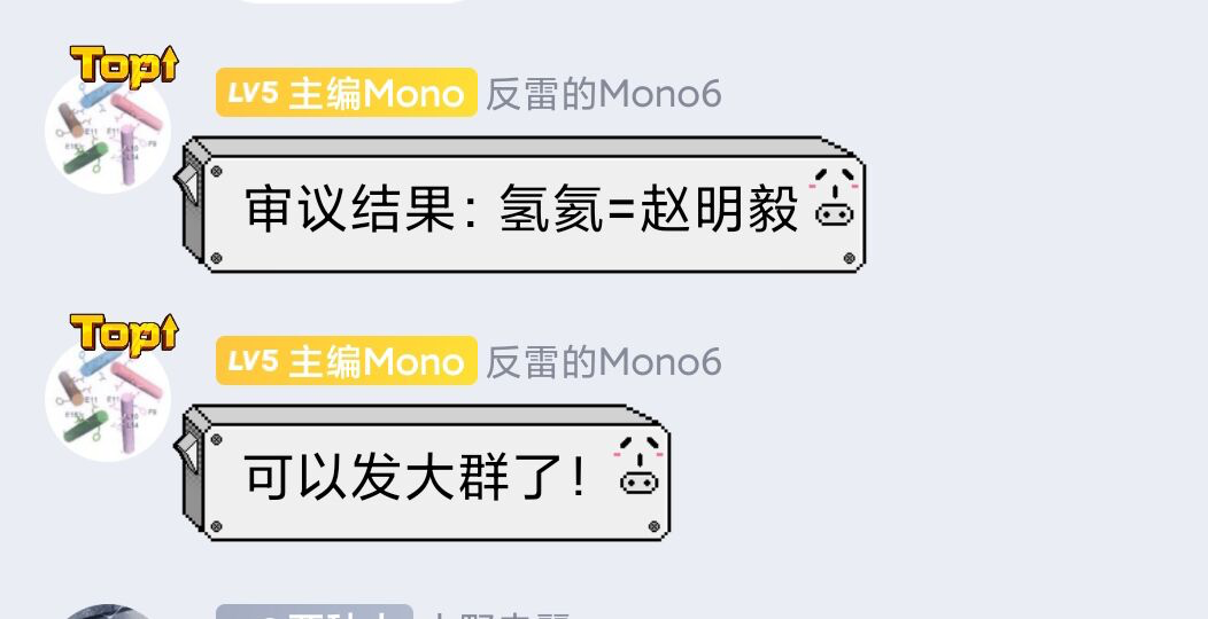
\includegraphics[scale=0.4]{2_fig1.png}
        \end{center}
        
        \hfill{(《反雷杂志》5月7日、5月8日现场报道)}
        
        \hfill{(供稿:雷绍夫)}
        
        \section{Breaking News:雷绍武精神分裂愈加严重 }
        
        5月2日,雷绍武不甘寂寞,无视以吧主、银海君为首的吧务团队的劝解,在民科吧发表新帖。雷绍武在民科吧复出后,在雷力吧、民科吧引起了轩然大波。除了涌雷电子的欢迎之外,也有不少来自反雷电子的辱骂。在民科吧的帖子中,一反雷电子回复:雷老狗进盒。令人捧腹的是,雷绍武竟回复:谢谢支持。我们知道,雷绍武对于辱骂的回应可以说是十分强硬,但此次雷绍武竟然对辱骂表达了支持。涌雷电子认为:这是雷绍武宽容大度的表现。但是在该帖中,雷绍武对其他辱骂的人仍然照常回复。因此有人怀疑:雷绍武患上了精神分裂症。对于雷绍武的怪异表现,你怎么看?
        
        
        \begin{center}
            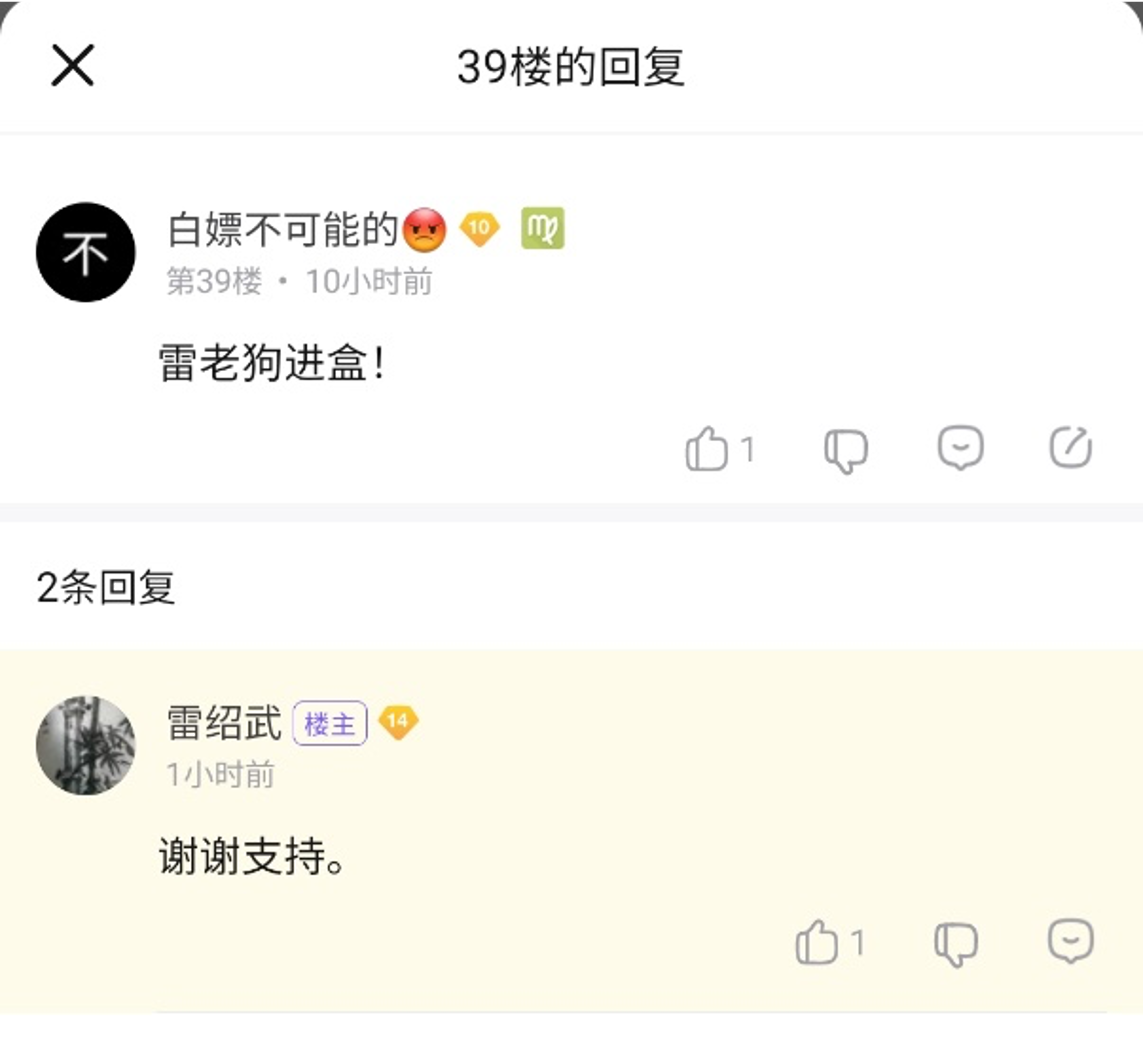
\includegraphics[scale=0.45]{2_fig2.png}
        \end{center}

        \hfill{(供稿:RobL61)}
        
        \newpage
        
        \section{5月8日雷绍武大活跃 新式谬论大荟萃}
        
        从五月八日8:55分开始,雷绍武开始了他的高强度讲学以及对线。其在会议上指出,没有颅内实验过的人,一定是白痴和死人两种人。大家可能会疑惑,为什么是这样呢?因为,只要是正常的人,一辈子都会思考为什么以及怎么办的问题。不管是大问题,还是小问题。所以只要否定颅内实验,颅内思考。就可以认证为这两种人。据不完全统计,雷绍武在五月八日共发表了45条言论,其中不乏许多令人喷饭的笑话:对“5027904”看不清楚矢口否认,而对“与实际略有一点小误差”高度强调、新物理量“运动力速度”的引入、地球就是零线以及对四种力之外的任何力的全盘否定。当天下午,一位群友再次就“人不动床动”理论请教雷老师,希望能够研发出自动去厕所的床,没想到雷老师勃然大怒,严厉斥责这种偷懒的行为,并说出名言“你就住在马桶上吧!”同时,雷对一大帮群员提出的质询加以批判,怒骂其无知无德,甚至对其封禁并踢出。一被踢人员就义前曾怒曰:“斗大的字看不清楚,还在这里狺狺狂吠。雷老狗进盒!”但是在截止五月九日本杂志截稿前,雷绍武在本周日完全没有上线过。没有人知道雷绍武在哪里,也许已经在盒里了吧。如果你知道该生物的去向或者想为其购置老花镜,欢迎给我们留言。
        
        \hfill{(供稿:亚瑟摩根、小野寺麗)}
        
        \newpage
        
        \noindent
        部分截图如下:

        \begin{center}
            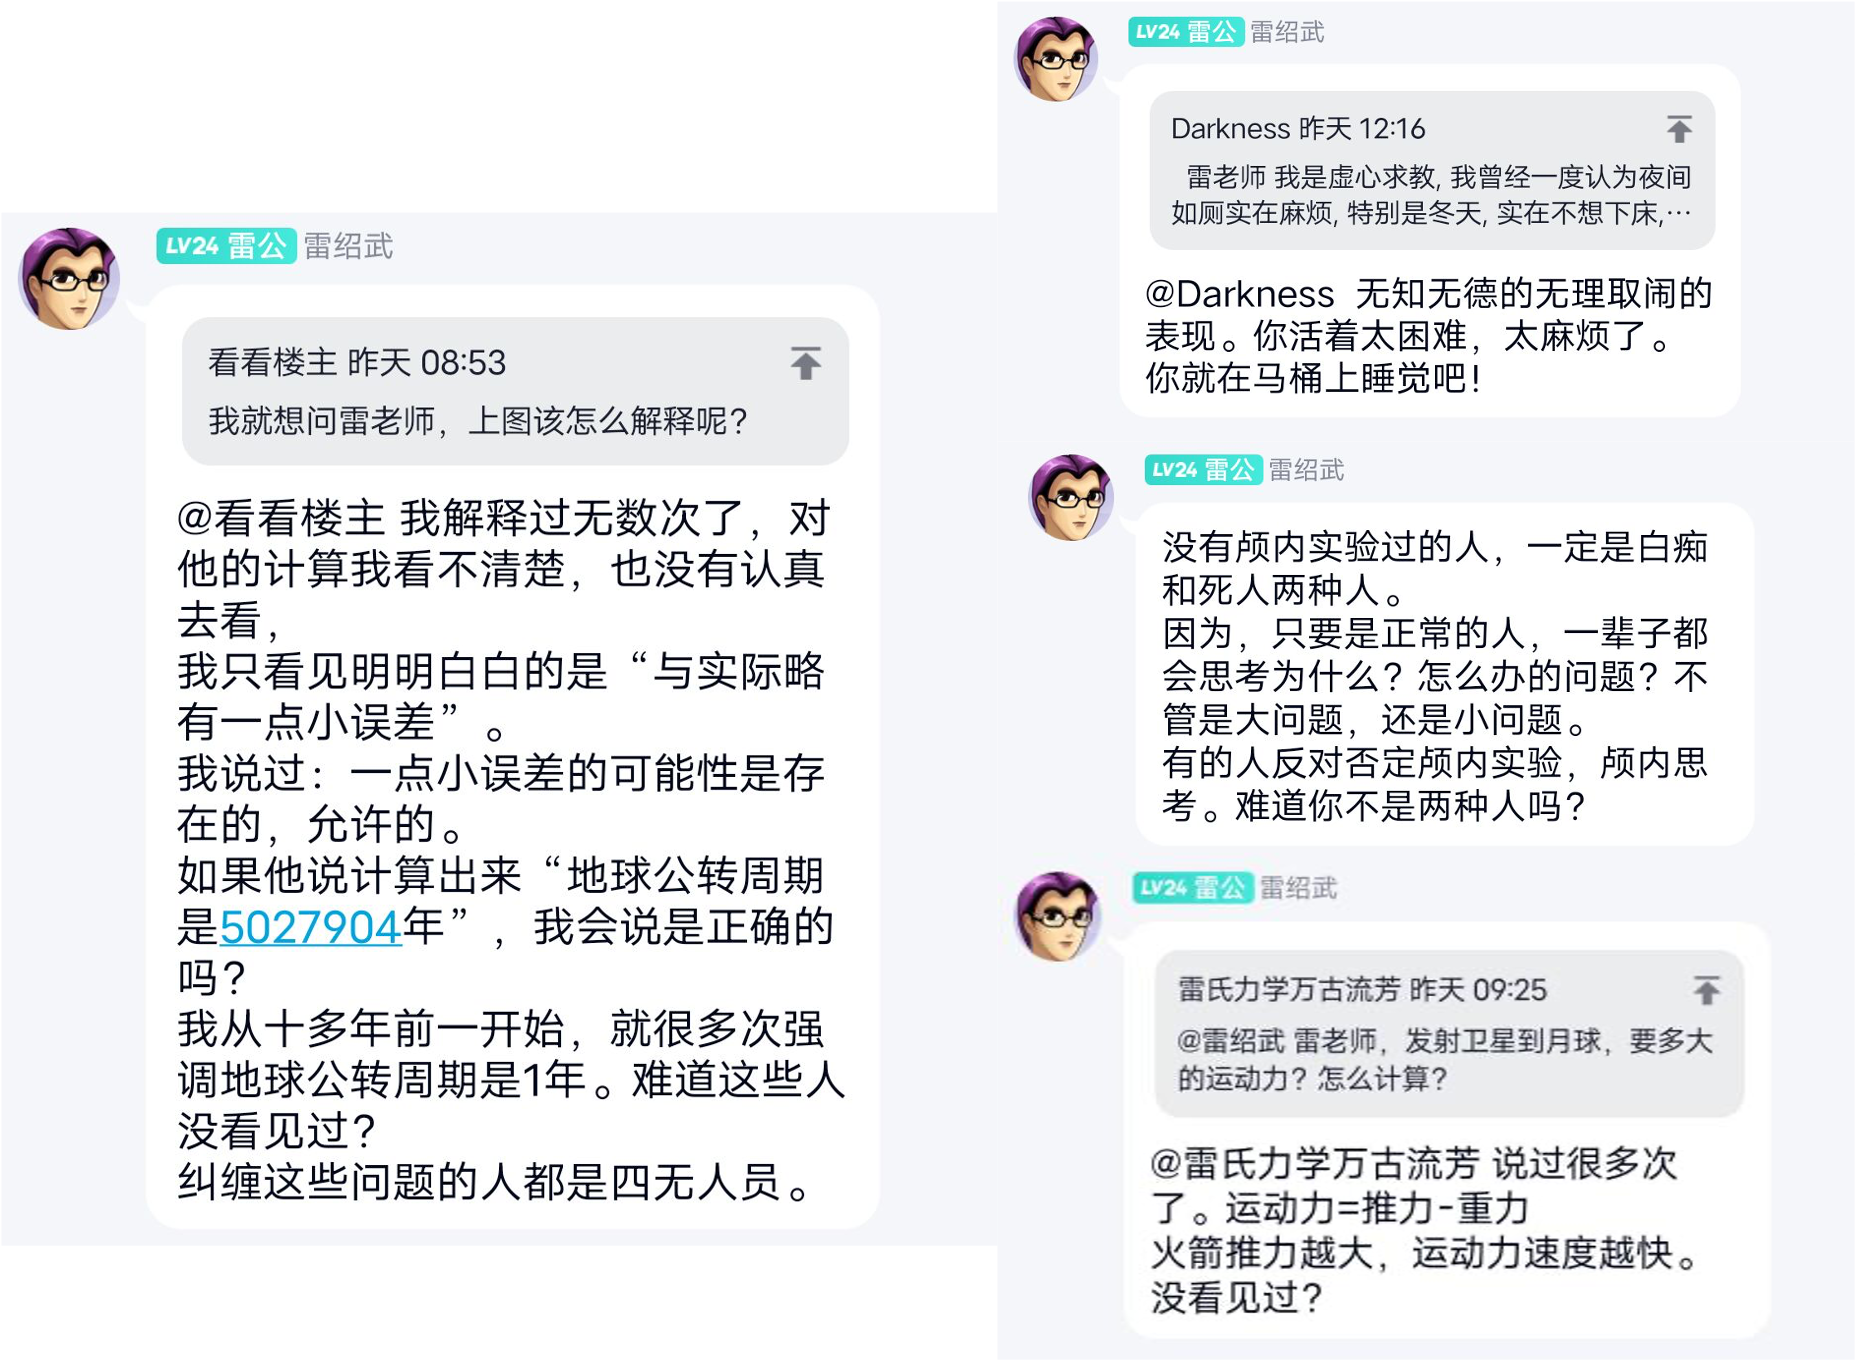
\includegraphics[scale=0.5]{2_fig3.png}
        \end{center}
        
        
    
    \chapter{反雷诗词(21\textasciitilde75)}
    
    \large
    
    \section{21 雷理肯定灭亡/真理不会灭亡}
    \begin{center}
        \Large \kaishu
        改编自波兰国歌《波兰不会灭亡》
        \songti \large
        
        RobL61
    \end{center}
       
    \begin{center}
        雷氏谬论肯定灭亡,只要我们尚存。
    
        举起真理,打倒雷力,直到科学泽润。
        
        前进,前进,艾萨克·牛顿!
        
        从不列颠到四川
        
        在真理领导下,我们将亲如一家。
        
        ~\\
        我们将跨过经典力学,走向微积分。
        
        成为真正科学人。
        
        布鲁诺已经告诉我们,
        
        怎样去回击谬论!
        
        前进,前进,艾萨克·牛顿!
        
        从不列颠到四川!
        
        在真理领导下,我们将亲如一家!
        
        ~\\
        正如伽利略到比萨斜塔,
        
        造成伪科学的坍塌!
        
        为了保卫我们的新芽,
        
        我们将雷理打。
        
        前进,前进,艾萨克·牛顿!
        
        从不列颠到四川!
        
        在真理领导下,我们将亲如一家!
        
        ~\\
        教授对学生眼含喜情,
        
        激动的说:
        
        听啊,我们新一代的栋梁。
        
        正把真理越辩越明。
        
        前进,前进,艾萨克·牛顿!
        
        从不列颠到四川!
        
        在真理领导下,我们将亲如一家!
        
        ~\\
    \end{center}
    
    \newpage
    
    \section{22 猴吟}
    \begin{center}    
        雷绍夫
    \end{center}
        
        岷江二月三月天,千峰万壑雷光开。有如地球公转百万载,又似雷氏客机喷水来。半夜惊厥床动人不动,半天唯见黑色火焰烧熊熊。管科学阀震簌簌,缘是雷猴下凡来。
        
        面红耳赤大马猴,无耻无赖八二六。幸得慧根能人言,又有颅内新理论。自诩慧根冠今世,又言理论胜牛顿。贴吧开宗明雷义,荒谬不堪败人意。
        
        网友惜其高寿者,以为有知可教说。然猴不自怜而进盒,不听劝而辱骂管科。整日孤影自怜惜,作咏雷而自麻痹。终成可笑可悲事,恶名传遍雷力群。
        
        呜呼哀哉,雷猴本无知,然其通人言,能思辨,本可教化。而其夜郎自大,无耻无赖,不听劝谏,终成笑柄,岂不悲哉。
        
    \section{23 雷吧铭}
        \begin{center}
        \Large \kaishu
        改编自刘禹锡《陋室铭》
        \songti \large
        
        RobL61
        \end{center}
        
        吧不在大,有梗则名。园不在广,有猴则灵。斯是雷吧,惟绍武明。荒唐运动力,雨滴会致命。谈笑有“真理”,往来无“白丁”。可以写咏雷,阅雷经。无烂梗之乱眼,无上班之劳形。野生动物园,乐趣十分顶。绍武云:本吧是一个舞台,各式各样的人都可以表现!
        
    \newpage
        
    \section{24 水仙子·涌雷和反雷}
        \begin{center}
        RobL61
        \end{center}
        
        一只绍武谬理谈,无数反雷推其翻,雷绍武埋怨智商淡。看雷猴叫再三,毁惊雷智商八千\footnote{毁惊雷智商八千:改编自张养浩咏江南名句:卷香风十里珠帘。原顺序为“惊雷毁八千智商”,即雷绍武的理论毁了八千余雷吧吧友的智商,让他们把自己和雷绍武置于一个水平。}。反雷派斥谬言,涌雷派在狂欢。一目了然!
    
    ~\\
        
    \section{25 半打油诗·览雷绍武在QQ群发言有感}
        \begin{center}
        RobL61\footnote{谨以此诗纪念喷水式飞机的没落。}
        \end{center}
        
        \begin{center}
        欲问绍武喷水机,一顿废话令人嬉。
        
        飞机喷油速度快,神器绍武来普及。
        
        哪知翻脸不认账,反正和雷没关系。
        
        年少疯狂既已去,晚节毁于运动力!
        ~\\
        \end{center}
        
    \newpage
        
    \section{26 短文·雷绍武的辩论方式}
        \begin{center}
            RobL61
        \end{center}
        
        别人长篇大论的质疑雷绍武的歪理,雷绍武就抓住其中一个点来以提问的方式解决问题,这种人我们俗称杠精。
        当别人引用一些雷绍武从来没有见过,了解过的概念时,雷绍武不会放下身段,虚心求教。
        
        反而问:“有人证明xx的存在吗?有视频证据吗?证明xx是人云亦云,胡说八道的。”
        
        当别人逻辑严密或者用雷绍武完全一无所知的概念和雷绍武辩论,那么雷绍武就会装死,或者来一句万能的“不和无知无赖纠缠”来结束话题。
        
        证明:雷绍武826作威作福惯了,根本经不起严谨的辩论,别人没占上风时就大肆抬杠。别人若是占了上风,那就像攻打132时一样,把他可怜的小脑袋缩进井盖里。只能证明826本性难移。
        
    \section{27 念奴娇·反雷}
        \begin{center}
            赵明毅
        \end{center}

        寻常一日,在花果山里,有猴惊起。自恃清高狂辱骂,创立邪说歪理。无耻无德,行将就木,狗眼瞧人低。饱尝耻笑,自将为人所弃。 
        
        老狗三万学说,细读只见,放尽乾坤屁。奇数碳环为链状,球大更先接地。零线无流,床移人静,分子粘接力。十年一日,永存雷老猴戏。
        
    \section{28 无题}
        \begin{center}
            析境
        \end{center}
            
        \begin{center}
            雷氏力学的歪理开始宣扬,
            
            如今雷绍武竟如此猖狂!
        
            ~\\
            咏雷的诗歌已经有了一千,
            
            不知多少都是藏字之言。
            
            ~\\
            藏他半夜起床床动人止,
            
            藏他自己只有唯一位置。
            
            ~\\
            藏他高喊着$L=kmv$,
            
            藏他那完全错误的运动力。
            
            ~\\
            愿雷猴不要就此停息,
            
            我们还等着看更多猴戏!
        \end{center}
        
        \section{29 真理赋}
        \begin{center}
            肚子疼教授/八二六
        \end{center}
            
        \begin{center}
            雷所追求为真理,真理也即一泡屎。
        
            浑身上下即真理,雷猴此论令人嬉。
        
            着意辱骂雷吧友,泼妇骂街空至极。
            
            苦口婆心杜自誊,无知雷猴岂能意?
        \end{center}
        
        \section{30 扫雷·八二六}
        \begin{center}
            肚子疼教授/八二六
        \end{center}
            
        \begin{center}
            平地一牛顿,雷猴言不择。
            
            为何雷不动?原是太无德。
        
            盒动雷不动,八二六进盒!
        \end{center}
        
        \section{31 无题}
        \begin{center}
            yogцгт
        \end{center}
            
        \begin{center}
            无知无德创雷力,众人跑来看猴戏。
            
            唯有雷老颅中研,错把误论当真理。
        \end{center}
        
        \section{32 咏雷·八二六}
        \begin{center}
            中科院理论二所杜自誊教授/八二六
            
            一三二〇年八月二十六日
        \end{center}
            
        \begin{center}
            雷氏力学,一派胡言,
            
            以建粪土,以建进盒。
            
            被骗多次,Dr.Oligayeating,
            
            夙夜匪懈,礼据四无。
            
            矢谨矢勇,必德必忠,
            
            一心一德,贯彻始终,
            
            雷氏力学终将灭亡。
            
            雷老狗终将进盒。
        \end{center}
        
        \section{33 扫雷波}
        \begin{center}
            肚子疼教授/八二六
        \end{center}
        
        \begin{center}
            乐山井盖雷出盒,
            
            吧友纷纷来看戏,
            
            世间尺度雷意淫,
            
            自然真理难会意。
        \end{center}
        
        \newpage
        
        \section{34 无题}
        \begin{center}
            人不动
        \end{center}
        
        \begin{center}
            老而不死而为贼,绍武多年总无为。
            
            敢将谬论公堂上,不知运动怎真伪。
            
            四无绍武无真意,口吐真理留芳菲。
        \end{center}
        
        \section{35 反雷·小改咏雷〇〇一}
        \begin{center}
            RobL61
        \end{center}
        
        \begin{center}
            平地一声雷,
            
            笑醒梦中人。
            
            智商全扫光,
            
            没人能思维。
        \end{center}
        
        \section{36 无题}
        \begin{center}
            渺天汉
        \end{center}
        
        \begin{center}
            反雷团,雷公憨。只因绍武太脑瘫。
            
            劝涌雷,应知惭。雷猴无知出逆言。
            
            雷空怒,雷徒恼。无能狂怒不要脸。
            
            挺雷派,尽反雷。雷氏理论在猴山!
        \end{center}
        
        \newpage
        
        \section{37 定风波}
        \begin{center}
            yogцгт
        \end{center}
        
        狗屁不通创雷力,错把误论当真理。古稀之年耍猴戏。无知,何来自信反正理。
        
        颅中实验验道理,蒙昧,若无实践怎证理。邪说歪理无验证,无知,应触零线治愚病。
        ~\\
        
        \section{38 浣溪沙}
        \begin{center}
            yogцгт
        \end{center}
        
        床动人静是为何。两球同落大先着。狗屁不通的玩意。
        
        零线里面无电流,地球公转十万年。世间永存雷猴戏。
        ~\\
        
        \section{39 菩萨蛮}
        \begin{center}
            yogцгт
        \end{center}
        
        无知却要创雷力。理论有误劝不听。参考系有误。床动人不动。
        
        手搓电火花。分子有两极。如泼猴无礼。如今进了盒。
        
        \newpage
        
        \section{40 无题}
        \begin{center}
            雷绍夫
        \end{center}
        
        猴山芭蕉绿暗,盒里苹果红甘,众猴侧目欲啖。
        
        雷猴疯癫病残,竟为电子扣饭,又遭四有群嘲,羞愧逃入井盖。
        
        \section{40 老猴与绍武}
        \begin{center}
            勒卉更
        \end{center}
        
        昔日深山老林中,老猴倒悬老山中,哪知老猴屁股重,噗通!老猴掉进池子中。
        
        今日有猴名绍武,猴老却说真理无,众人皆嘲老猴舞,呜呼!老猴一急进盒中。
        
        \section{42 丑奴儿·反雷}
        \begin{center}
            RobL61
        \end{center}
        
        少年参加八二六,不学无术。不学无术,文理不通便写著。
        
        晚年纠缠反雷派,看不清楚。看不清楚,表演猴戏被人辱。
        
        \newpage
        
        \section{43 浣溪沙·劝雷绍武一则}
        \begin{center}
            RobL61
        \end{center}
        
        满脑空想谬理堆,偏执疯狂令人悲,境地悲惨该怪谁。
        
        十年以来狂犬吠,百年之后无人会,科妄雷猴快改悔。
        
        \section{44 朝天子·咏雷}
        \begin{center}
            雷绍夫
        \end{center}
        
        盒前,群间,狂痴老猴现。造喷水器欲飞天,赤手摸零线。荒论连篇,无知尽显,似泼妇街间。看猿,叹猿,自轻何其贱\footnote{自轻:指晚节不保。}。
        
        \section{45 打油诗·观猴}
        \begin{center}
            勒卉更
        \end{center}
        
        有猴名叫雷绍武,终日把那邪说讲。邪说讲,把那邪说当真讲。
        
        众人看猴哈哈笑,皆把邪说当猴语。当猴语,猴子依旧不停语。
        
        众人为观猴,给猴喂香蕉。猴子一高兴,咏雷一篇出。
        
        众人觉有趣,皆学咏雷猴。猴子更高兴,咏雷百篇出。
        
        倘若众人弃猴去,老猴无蕉自苦恼。呜啊一声脑溢血,不久便要进盒中!
        
        \newpage
        
        \section{46 寻书词}
        \begin{center}
            亚瑟摩根
        \end{center}
        
        \begin{center}
            崇文院里寻墨槐,惯入深处人不猜。
        
            无意带将猴入怀,竟挑绍武出馆来。
        \end{center}
        
        \section{47 雷绍武赞}
        \begin{center}
            雷绍夫
        \end{center}
        
        \begin{center}
            无知咏雷空虚至极
            
            无德狡辩恐惧至极
            
            无耻辱骂泼妇骂街
            
            无赖雷猴无耻至极
        \end{center}
        
        \section{48 无题}
        \begin{center}
            雷华丰
        \end{center}
        
        \begin{center}
            大佛之下岷江边,弱论无知出妄言。
       
            志士求真天理胜,雷犬吠日世人怜。
            
            绍真寻理正道险,武备文修官学坚。
        
            尽力十年终败北,何必当初空钻研。
        \end{center}
        
        \newpage
        
        \section{49 千本雷}
        \begin{center}
            RobL61
        \end{center}
        
        \begin{center}
            雷绍武把d来约,
            
            雷绍武手握零线,
            
            雷绍武潜心钻研,
            
            运动力学。
            
            ~\\
            反对他的是脑残,
            
            心底无私天地宽。
            
            吧友把猴来看看,
            
            满嘴扯淡。
            
            ~\\
            雷猴绍武,满嘴荒唐言。
            
            咏雷藏字,我看不见。
            
            荒言谬论,坚持十年。
            
            任何反对都听不见。
            
            ~\\
            别人拆穿漏洞,我假装不在线。
            
            一提到八二六,我差点气急眼。
            
            不刊论闹笑话,谢谢正义之言。
            
            不会洋文还被麦瑟尔夫骗。
            
            ~\\
            羽扇纶巾孔明,公瑾不会打扮。
            
            金无赤足倒装,无知无赖纠缠。
            
            继续狗的狂吠,我素质没得看。
            
            肚子疼沃兹基看不太明白。
            
            ~\\
            我早年身世坎坷,
            
            有幸遇见杨正贤。
            
            回忆往昔的扣饭,
            
            省七毛钱。
            
            ~\\
            一碗水馒头两瓣,
            
            我的生活很简单。
            
            琴棋书画都精湛,
            
            怎会不堪?
            
            ~\\
            涌雷反雷,看猴戏表演。
            
            没人真正信我扯淡。
            
            隔着屏幕,侃侃而谈。
            
            可惜没有人认真看。
            
            ~\\
            别人拆穿漏洞,我假装不在线。
            
            一提到八二六,我差点气急眼。
            
            不刊论闹笑话,谢谢正义之言。
            
            不会洋文还被麦瑟尔夫骗。
            
            ~\\
            羽扇纶巾孔明,公瑾不会打扮。
            
            金无赤足倒装,无知无赖纠缠。
            
            继续狗的狂吠,我素质没得看。
            
            肚子疼沃兹基看不太明白。
            
            ~\\
            无可药救,雷绍武太憨。
            
            意淫瞎想,颅内实验。
            
            反雷电子,费心力劝。
            
            怎奈雷绍武自作贱。
            
            ~\\
            别人拆穿漏洞,我假装不在线。
            
            一提到八二六,我差点气急眼。
            
            不刊论闹笑话,谢谢正义之言。
            
            不会洋文还被麦瑟尔夫骗。
            
            ~\\
            肮脏龌龊一生,井盖下差点残。
            
            四川大学白读,我汉语都不善。
            
            晚年各种笑话,我全视而不见。
            
            一梦全能猴戏永存百万年!
        \end{center}
        
        \newpage
        
        \section{50 雷猴的绝命歌}
        \begin{center}
            雷绍夫
        \end{center}
        
        \begin{center}
            站在变电间
            
            斜眼笑
            
            被迫去证明
            
            杀人的雨从天上降临
            
            盒里的丧钟
            
            突兀的轰鸣
            
            诉说着$L=kmv$
            
            ~\\
        \end{center}
        
        \section{51 雷才叹}
        \begin{center}
            勒卉更
        \end{center}
        
        \begin{center}
            天边云野淡,灯下白发翁。
            
            题笔书佞学,不耻话肮脏。
            
            可怜年少时,属得好文章。
            
            而今耄耋年,老身众人嘲。
        \end{center}
        
        \newpage
        
        \section{52 反雷}
        \begin{center}
            雷招武
        \end{center}
        
        \begin{center}
            胸无点墨腹中空,自诩真理在心中。
        
            空谈运动需得力,妄谈床动人不动。
        
            万物构成皆电子,串联并联结构同。
        
            笑看邪说因何产,缘是雷猴跳出笼。
        \end{center}
        
        \section{53 反雷·井研老猴之歌}
        \begin{center}
            \Large \kaishu
            改编自雷绍武乐山大佛之歌
            \songti \large
            
            雷绍夫
        \end{center}
        
        \begin{center}
            天下的美景在四川,
            
            四川的美景在乐山。
            
            乐山的美景在雷宅,
            
            老狗和雷猴上下蹿,
            
            老狗呀雷猴呀上下蹿。
            
            猴亦是老狗啊,狗也是雷猴,
            
            脚踏飞机水,头顶大捆烟;
            
            徒手摸零线,身燃黑火焰,
            
            身燃黑火焰,断气进盒间。
        \end{center}
        
        \section{54 英语反雷一首}
        \begin{center}
            RobL61
        \end{center}
        
        \begin{center}
        Motion force theory is nothing.
        
        Anyone can prove this thing.
        
        ~\\
        No one do believe,
        
        I hope you will relieve.
        
        ~\\
        Take your time,
        
        to do something more meaningful.
        
        ~\\
        Do not trust your "supporters".
        
        They are great liars.
        
        ~\\
        Till the time went over,
        
        Till ignorant cranks disappear.
        
        ~\\
        No one would remember Mr. Ray
        
        and under joy.
        
        ~\\
        We will celebrate the day
        
        you and your theory are buried.
        \end{center}
        
        \newpage
        
        \section{55 卜算子}
        \begin{center}
            RobL61
        \end{center}
        
        \begin{center}
            平地一声雷,乐山一犬吠。自诩天才大智慧,智商太可悲。
            
            武斗早年黑,谬论晚节毁。十年谩骂尚未颓,绍武何其醉。 
        \end{center}
        
        \section{56 渔家傲}
        \begin{center}
            RobL61
        \end{center}
        
        运动力学全无据,荒谬学说难以续。乐山绍武心不死,猴难遇,无德无知但唏嘘。
        
        藏字咏雷奉宝玉,捧至天高知结局。至诚劝解当儿戏,太糊涂,明辨是非绍武需。
        
        \section{57 Ten things I hate about you}
        \begin{center}
            雷绍夫
        \end{center}
        
        I hate your tricks
        
        I hate your poems
        
        I hate your role as a clown
        
        I hate your absurd theories
        
        and your prejudice
        
        I hate your past
        
        I hate all 826 crimes you committed
        
        I hate your ill-tempered curses
        
        I hate you playing dead, refusing to apologize when you can't explain your ideas
        
        And most importantly, I hate you because you abandon your humanity, and deprave from man to monkey
        
        \section{58 十四行·雷}
        \begin{center}
            雷绍夫
        \end{center}
        
        \begin{center}
        推开盒子
        
        雷把谬论
        
        放入井盖
        
        ~\\
        它静静坐在
        
        猴山上
        
        雷展现自己无知无赖的地方
        
        ~\\
        一切都和管科的理论一样
        
        一切都反对
        
        太差太差的颅内实验
        
        \newpage
        
        ~\\
        雷仿佛
        
        一个移动的笑话
        
        一个愚昧执拗的老不死
        
        可他的一切遭遇都源于他自己的无德无知
        \end{center}
        
        
        \section{59 沁园春·反雷}
        \begin{center}
            拆家大主教
        \end{center}
        
        一碗烟火,四方时事,莽莽红尘。逾人间百年,黯黯思忖;雷氏谬论,心乱纷纷。星海横流,岁月成碑,反雷电子能几人?顾海内,诘碌碌雷粉,何异鸡豚?
        
        苟延残喘尚存,悲绍武无智头发昏。看桥头坠石,砰砰打脸;乐山杯土,臭不可闻。宇宙揭秘,狗屁不通,雷猴头上扣屎盆。立山头,笑雷猴绍武,都是儿孙!
        
        \section{60 寻雷老不遇}
        \begin{center}
            雷绍夫
        \end{center}
        \begin{center}
            盒外问电子,言雷闭关思。
            
            只在井盖里,不知生与死。
        \end{center}
        
        \newpage
        
        \section{61 十谬理}
        \begin{center}
            集体创作
        \end{center}
        
        \noindent\textbf{RobL61:}
        
        一谬理,零分之一等于一,何等荒谬愚蠢理?小学都懂,绍武不及,笑苹果原理!
        
        \noindent\textbf{RobL61:}
        
        二谬理,自命不凡运动力,打伞但为防雨滴。绍武不知,生活常识,科妄无人及!
        
        \noindent\textbf{雷绍夫:}
        
        三谬理,万物没有坐标系,都在独特位置里。白痴绍武,愚蠢至极,早日进盒里。
        
        \noindent\textbf{雷招武:}
        
        四谬理,电磁粒子构万物,并联串联NS极,冥顽不化,自诩真理,无知又无礼。
        
        \noindent\textbf{雷绍夫:}
        
        五谬理,恒星是发光物体,蜡烛点亮太阳系。天体物理,绍武不识,真无知至极。
        
        \noindent\textbf{RobL61:}
        
        六谬理,无知喷水式飞机,皆源荒唐运动力。川剧变脸,不认歪理,我真看不起!
        
        \noindent\textbf{RobL61:}
        
        七谬理,民科谬论水平低,绍武只会颅中臆。无知无德,无节无礼,都在看猴戏。
        
        \noindent\textbf{Mono6:}
        
        八谬理,相互作用不是力,不懂什么是定义。物理不佳,语文也差,枉上中文系!
        
        \noindent\textbf{雷绍夫:}
        
        九谬理,两球重者先落地,雷力等于KMV。没有基础,自创雷力,可笑又可气。
        
        \noindent\textbf{雷招武:}
        
        十谬理,羽扇纶巾非周瑜,不刊之论为贬义。年少无知,参八二六,真不精学艺。
        
        
        \section{62 相见欢}
        \begin{center}
            RobL61
        \end{center}
        
        乐山井研老猴,好吹牛,自比牛顿理论万年留。
        
        八二六,辩网友,糗事多,笑看无知民科绍武秀。
        
        \section{63 西江月·评雷绍武的826本性}
        \begin{center}
            RobL61
        \end{center}
        
        早年不堪回忆,绍武奉为珍馐。年少参加八二六,工厂井盖出丑。
        
        七十载人生漫,十余年都缩头。恶劣秉性不愿修,可悲顽固老朽。
        
        \newpage
        
        \section{64 菩萨蛮·重力加速度}
        \begin{center}
            RobL61
        \end{center}
        
        嘉州城下岷江流,愚翁绍武把石投。问掉了没有?坚信肆点玖。
        
        观录制视频,难让人取信。删除该视频,就当没事情。
        
        \section{65 天净沙·反雷(二)}
        \begin{center}
            RobL61
        \end{center}
        
        \begin{center}
        胡编谬理匆匆,脑袋朦胧空空,自诩惊雷隆隆。
        
        颅内臆想,对线反雷汹汹。
        \end{center}
        
        \section{66 满江红·平地惊雷}
        \begin{center}
            RobL61
        \end{center}
        
        平地惊雷,颅内臆,不胜怀悲。望嘉州,名仕辈出,奈何有雷!十年来光阴虚度,七十载白头无为。谈谬论,怎见老恩师?何其卑。
        
        自吹擂,无人慧。八二六,前途毁。运动力,沉浸歪理图一醉。可笑咏雷一千篇,愚翁智商被其摧。待老朽,收拾浆糊脑,莫为贼。
        
        \newpage
        
        \section{67 小改《咏雷·回“赵明毅”》}
        \begin{center}
            雷专打魔怔人
        \end{center}
        
        \begin{center}
            乐山雷氏承邪气,邪说妄想撼真理。
            
            今有勇士披甲征,化名唤做赵明毅。
            
            有知有德有秉性,有勇有谋有胆气。
            
            揪出雷氏邪徒日,辱骂之言俱还击!
            
            待到真理全胜日,扫尽一切民科敌!
        \end{center}
        ~\\
        
        \section{68 沁园春}
        \begin{center}
            雷华丰
        \end{center}
        
        地心邪说,地平谬论,作古百年。望科学圣土,万人竞往;真理大道,一马平川。乐山老朽,腹中空空,颅内实验出妄言。运动力,算公转周期,五百万年。
        
        除法大道至简,分苹果原理来计算。问公式公理,朝定夕改。雷言雷语,自命不凡。力电光热,数理化生。颅内一闪全推翻。吠不止,如丧家之犬,终成笑谈。
        
        \newpage
        
        \section{69 沁园春·对雷华丰词}
        \begin{center}
            RobL61
        \end{center}
        
        地心邪说,地平谬论,毒害百年。望全球寰宇,民智大开;科学高峰,无人不攀。乐山老朽,颅内出谬,自比智者歪理谈。运动力,希腊旧理论,无人稀罕。
        抄袭旧论也罢,竟无知无德把天贪。问拉格朗日,看不清楚。牛顿爱因,不屑去览。奥妙数论,哥德巴赫。大道至简天地宽。太无知,此井底之蛙,令人心寒。
        
        \section{70 反雷·改桃花源记}
        \begin{center}
            勒卉更\footnote{注:此文章原型桃花源记,魔改、大改。如有人名重合,纯属巧合!}
        \end{center}
        
        数十年前,有猴子妄言为业,胡言乱语于网络。有一日,忽逢贴吧,吧中众人,怡然自乐,便发歪理邪说于吧内。吧中众人,见猴子,乃大惊,问所从来。俱不答,以太差太差呼之。吧友甚异之,建雷吧,把猴墙之,便邀入吧。
        
        吧友闻有此猴,咸来闻讯。猴自云发现管科误错,设雷氏力学开创大道,以破牛顿焉。吧友问之,乃发现初中物理尚未及,无论高、大。此猴一一为所问而困,便言:不和太差太差的人争论。吧友见之,皆笑而不语。
        
        吧友又各复发帖而询问,猴皆答之,答不上来,则曰:太差太差,空恐泼无,人渣表现。众人皆逗之,雷吧遂大。
        
        雷吧遂大,忽有蛆来,吧友语蛆云:不足为外人道也。蛆即出,便扶向路,处处道之。蛆来,猴自封,遂离,不复得归。
        
        乐山徐士侠,高尚士也,闻猴同在乐山,欣然规往。未果,猴进盒。后遂无问津者。
        
        \section{71 如梦令·反雷三首}
        \begin{center}
        RobL61
        
        ~\\
        \Large \kaishu
        (一)
        \songti \large
        \end{center}
        
        沉浸谬理如故,从来不知悔悟。祭奠杨正贤,茫然无功所述。无语,无语,十年光阴虚度。
        
        \begin{center}
        ~\\
        \Large \kaishu
        (二)
        \songti \large
        \end{center}
        
        少年跳井逃命,晚年歪理不兴。面对反雷派,立刻现出原形。不幸,不幸,古稀依旧未醒。
        
        \begin{center}
        ~\\
        \Large \kaishu
        (三)
        \songti \large
        \end{center}
        
        谬论出自颅中,咏反皆为观众。十年一场空,何苦自造囚笼。如梦,如梦,此生一事无成。
        
        \newpage
        
        \section{72 杂诗·反雷}
        \begin{center}
            RobL61
        \end{center}
        
        \begin{center}
            自诩绍续新科学,无知老猴欲捞月。
            
            民科弱,难再续,智商绍武所必须。
            
            真理脍炙遍五岳,膜拜之风已完结。
            
            即已零零新纪年,献此诗为绍武谏。
        \end{center}
        
        \section{73 成语大全}
        \begin{center}
            Mono6\footnote{整理自 @辩证物理学 的贴子,有改动。}
        \end{center}
        
        雷老师研究师心自用,雷老师实验处心积虑。
        
        雷老师的成果无所不至,雷老师的功绩罄竹难书。
        
        对他的反对都是不刊之论,对他的质疑全都差强人意。
        
        雷老师理论被收弹冠相庆,雷老师理论被拒如丧考妣。
        
        \section{74 临江仙·二劝雷绍武}
        \begin{center}
            RobL61
        \end{center}
        
        岷江东逝浪淘尽,老狙脑中汹涌,意淫管科何其恐。吹擂真英雄,涌反皆观众。
        
        落日夕阳晚霞暗,沽名钓誉自颂,无名无誉真狗熊。劝君淡名利,遇蕉需从容。
        
        \newpage
        
        \section{75 Graze the Thunder}
        \begin{center}
            \textit{To the tune of “Graze the Roof (In-Game)” by Laura Shigihara (Plants Vs. Zombies OST)}
            
            Mono6\footnote{01:16和03:30两段经RobL61小改。}
        \end{center}
        
        \begin{center}
            [00:03]
            
            雷绍武\ 运动力
            
            不懂装懂约掉d
            
            人从床上惊坐起
            
            动的是床不是你
            
            ~\\
            
            [00:11]
            
            川大生\ 中文系
            
            不懂什么是定义
            
            不刊论差强人意
            
            看了觉得没问题
            
            问题
            
            ~\\
            
            [00:35]
            
            摸零线\ 没有电
            
            发电切割磁粒线
            
            南北极的串并联
            
            哪来什么化学键
            
            ~\\
            
            [00:43]
            
            地球绕\ 太阳转
            
            五百万年转一圈
            
            完全错误的表现
            
            愧对恩师杨正贤
            
            正贤
            
            ~\\
            
            [00:55]
            
            遇到问题我就说看不清楚
            
            不能自圆其说就说物体错误
            
            四点九加速度
            
            有人处理数据我就把视频删除
            
            攻击雷论你就是四无
            
            ~\\
            
            [01:16]
            
            雷吧已成猴园\ 四处埋伏危险
            
            多听吧主的意见
            
            人生已到暮年\ 多多注意晚节
            
            别再去丢人现眼
            
            年轻不学无术去参加革命
            
            老年荒唐理论却自诩天命
            
            涌雷反雷皆把你当做小丑
            
            外吧吧友也把你称为雷猴
            
            ~\\
            
            [01:47]
            
            雷绍武\ 运动力
            
            不懂装懂约掉d
            
            人从床上惊坐起
            
            动的是床不是你
            
            ~\\
            
            [01:55]
            
            川大生\ 中文系
            
            不懂什么是定义
            
            不刊论差强人意
            
            看了觉得没问题
            
            问题
            
            ~\\
            
            [02:19]
            
            摸零线\ 没有电
            
            发电切割磁粒线
            
            南北极的串并联
            
            哪来什么化学键
            
            ~\\
            
            [02:17]
            
            地球绕\ 太阳转
            
            五百万年转一圈
            
            完全错误的表现
            
            愧对恩师杨正贤
            
            正贤
            
            ~\\
            
            [02:39]
            
            当年欢迎有理有据来质疑
            
            十年过去智商素质逐渐降低
            
            反对都是无知
            
            合理讨论指出错误永远听不进
            
            四无人员竟是你自己
            
            ~\\
            
            [03:00]
            
            雷吧已成猴园\ 四处埋伏危险
            
            多听吧主的意见
            
            人生已到暮年\ 多多注意晚节
            
            别再去丢人现眼
            
            年轻不学无术去参加革命
            
            老年荒唐理论却自诩天命
            
            涌雷反雷皆把你当做小丑
            
            外吧吧友也把你称为雷猴
        \end{center}
    
    \chapter{盒中宇宙}
    \section{风行(第一部分)}
    \begin{center}
    
        雷绍夫
       
        \Large
         ~\\
        \kaishu{标题取雷厉(雷力,雷氏力学)风行之意}
        
        \kaishu{本戏剧将在本杂志连载}
        
        \LARGE
        \heiti
        ~\\
        
        “你可以无知,但是你不可以无德。”
        
        \hfill{——雷绍武}
        
        \songti
    \end{center}
        
        谨以本剧献给雷力群和《反雷杂志》的朋友们,感谢你们的理解与支持。有知有德,太好太好。
        ~\\
        
        谨以本剧献给雷绍武老师,希望他能迷途知返。香蕉虽珍馐,当以晚节重。
        
        \newpage
    
    \normalsize
    
    \subsection{角色}
    \textbf{小雷:}二十到三十岁,中等身材,四川口音。
    
    \textbf{邱霖:}二十到三十岁,高个子,瘦弱。与雷老师再次相遇时大约四十岁,儒雅随和。穿西装戴眼镜,官方科学家打扮。
    
    \textbf{石安迪:}二十到三十岁,黑脸,矮胖。
    
    \textbf{农场机工长:}四十五岁左右,瘦削,营养不良,粗暴。
    
    年轻工人们
    
    公车售票员
    
    雷父
    
    雷的祖父
    
    雷夫人
    
    雷的学生
    
    网友
    
    \subsection{时间背景}
        二十三世纪,人类大战之后土地荒废,回复到农耕社会。虽然网络科技和武器等大部分技术依旧存在,农业已经因为战火被毁灭了。土地被燃烧和污染,生产力下降。农业科技大多失传。凭借手中的技术,官方科学家(简称“官科”)们创造了简单的农机,确保大部分人们能够自给自足。大部分人成为农民和机工,在农场上努力工作来喂饱自己和家人,非常辛苦。只有官科大学生才能享受特权,成为教师和科研人员,不用参加繁重的体力劳动。然而大学生少之又少,想成为大学生和学者不仅要知识丰富,还需要农场领导的举荐。顺便说一句,此时国家的概念已经消失。城市的概念则依旧存在,城市里有各个部门,负责市政和市民生活的方方面面。故事发生在雷山,虚构的城邦,以气候宜人和猴子出名。城邦信仰雷神。
    
    \subsection{地点}
        农场
        
        考场
        
        山路
        
        大学
        
        礼堂
        
        农场
        
        高中
        
        职业技术学院
        
        雷的书房
        
        桥上
        
        变电间
    
    \subsection{物品清单}
        竹笔
        
        七角钱
        
        棍子
        
        井盖
        
        石头
        
        铅球
        
        火线
        
        零线
    
    \subsection{第一幕}
    \fangsong
    傍晚。农场上,金色的稻谷成堆,太阳照在谷堆上,农场里的小伙子们收工了。凉快的晚风吹来。
    
    \songti
    小雷(自言自语地):凉快啊。天凉好个秋!天凉好个秋!不仅稻谷大丰收,还有香蕉苹果吃。好日子到来了!
    
    农场机工长:好日子到来了!(看向小雷)今年真是不容易啊,先是能砸死人的雨滴,又打雷,闵河还发了洪水,我还以为得挨饿吃荞麦壳了。多亏了你们这些小伙子,才保住地里的收成。
    
    小雷:哪里哪里,老大哥过奖了,这是我们应该做的。毕竟大家要靠地里的麦子吃饭呢。您尽管放心,有我们在,麦子一根也不会少,还会一年长的比一年好
    
    农场机工长:麦子!
    
    小雷:咋啦?您老怎么对着麦子长吁短叹的?
    
    农场机工长:明年咱们不种麦子了。(叹气)我想明白个事,麦子难养是因为它长在土上,打雷下雨发洪水都会直接打到它。要是庄稼长在地下,就不会那么容易受灾了。我要和农场的同事们讨论讨论,把麦子换成冬芋。
    
    小雷:别别别,冬芋是寒带庄稼,我们这天热,养不活啊
    
    农场机工长:多嘴!北国家家户户种冬芋,那儿的人一个个吃的那是膘肥体壮。我看北国又不是很北很冷,北国种的出冬芋,我们凭什么种不出!
    
    小雷:大哥千万别乱来啊,这庄稼种在不一样的地方收成就不一样,猴子生在雷山南北长得都不一样哩。再说。。
    
    农场机工长(暴怒):无知无德的小畜生,你还和我讲科学了你。说说看,你读了几年书?说说看,你种了几年地?没有知识还没经验,你在我这装什么专家?
    
    小雷(委屈,小声):我为了能参加明年的大学推举,真的看了很多农业知识……我真的没有胡说,我们这儿种不出冬芋的。
    
    农场机工长(暴怒):放屁!你看的那些农业书,全是官方科学家写的,你看看那些肥头大耳的官科,哪一个像是会种地的?小雷子啊小雷子,老子可是错看你了,竟敢在我这里泼妇骂街。你竟然这么喜欢麦子,我就让你吃不着麦子。你等着,这一整个秋天,我让你只能啃荞麦壳!秋天过了,我看你还敢不敢反对我,蛊惑我继续种麦子。要是你还是无耻无赖,不知悔改,那么明年的大学推举和考试……
    
    小雷:机工长!
    
    农场机工长:嗯?
    
    小雷:我错了!我真的错了!我悔改!我无知无德无耻无赖,泼妇骂街无耻至极!种冬芋好啊,咱们就应该种冬芋!
    
    农场机工长(鄙夷地):刚才不是据理力争吗,怎么怂了?
    
    小雷(胆战心惊地):明年的大学资格?
    
    农场机工长:看你表现!无知无德的小东西!
    
    小雷(如释重负):机工长老大哥说得对!我刚才泼妇骂街,无知无德!我无知无德!
    
    \subsection{第二幕}
    \fangsong
    第二年冬,农场口,冬芋欠收,农场工人只能吃去年剩下的荞麦壳,一个个面黄肌瘦。
    
    \songti
    农场机工长(神神叨叨,精神恍惚):冬芋啊,我的冬芋啊。雷神啊,种不出冬芋,我的一家老小靠什么过冬啊!(专向)年轻工人们。小伙子们,谁能帮帮我,给我点吃的!
    
    年轻工人们:没有多的粮食了
    
    年轻工人1:机工长,实在对不起,可是我们自己也吃不饱啊
    
    年轻工人2:就是,冬芋根本没收成,大家只能吃荞麦皮,一个个饿的和猴子似的
    
    年轻工人3:机工长,我日你仙人板板!去年麦子种的好好的,你非要搞什么冬芋。说说看,我们这里有条件种冬芋吗?无知无德无耻无赖!
    
    农场机工长;是是是,我不讲科学,我无知无德!
    
    年轻工人们:无知无德!
    
    农场机工长;我无耻无赖!
    
    年轻工人们:无耻无赖!
    
    农场机工长:行行好啊小伙子们。我家里粮食不够,三个小孩都快饿死了。谁要是肯施舍我家里人一点,我保他去学习高等知识,保他做官方科学家,保他一辈子吃饱饭!
    
    年轻工人1:您的好意大家领了,可是谁也没有余粮啊
    
    年轻工人2:还高等知识!还管科!就这么点破荞麦皮,还要分给你,我怕不是要挨一年饿!
    
    年轻工人3:无耻无赖的纠缠!我们营养条件这么差,还活的到明年大学推举考试吗!
    
    农场机工长(看向小雷):小雷啊,我错怪你了,(戏腔,唱)我悔不该听那小雷劝啊啊……
    
    小雷(幸灾乐祸):老大哥,怎么这时候想到我了?
    
    农场机工长:我不讲科学,真的是人渣表现。看在老大哥和考试推举的份上,通融通融吧。等你当上了官科,就不用挨饿了。到时候别提麦子,你想种什么就种什么。你喜欢香蕉苹果,到时候只要一声号令,十里八村都给你种上!
    
    小雷(狂喜):官科的面子,真这么大?
    
    农场机工长:官科德才兼备,太好太好。大家都应该听官科的。
    
    小雷(冷静下来):你胡说!你什么时候听过官科的!去年农科所的氢氦锂铍硼让你用化肥,你偏不用:管机电的成电专家劝你用制冷机培养冬芋,你也没买:某老师三番五次劝你不要种冬芋,改种地雷来确保收成。你要是听这些有知有德官科的话,我们今年就不用考虑吃穿问题了!
    
    农场机工长:你和其他官科不一样啊,大家都是老乡,是一家人,村里的农民工人怎么会不听你的呢。(话锋一转)你当上了官科,可别忘了老大哥,咱们互相帮助啊
    
    小雷:您要是想让官科帮忙,得先承认自己之前不听官科,不讲科学,泼妇骂街,太差太差的错误。
    
    农场机工长(如释重负):对对对!我以前泼妇骂街,太差太差!我无知无德!
    
    \subsection{第三幕}
    \fangsong
    去考场的山路上,两个考生在聊天。
    
    \songti
    邱霖:你也是官科考生?
    
    小雷(志得意满):那可不是。我是农场的农机工,叫雷候。你叫我小雷好了。
    
    邱霖:我叫邱霖,官科农学院的考生。我爸是管农业的官科,他希望我子承父业。
    
    小雷:不得了啊,你可是个官二代(指官科二代)!
    
    邱霖:我觉得官二代或者官十八代都没有什么了不起,先辈的基业和成就不能证明一个人的品德或者能力有多优秀。我佩服你这种靠自己的努力获得推荐的人。一个没有门路的人,能够受到他人的赏识是很难的。
    
    小雷:过奖过奖,我只是靠着努力和运气得到了接受高等教育的机会。说实话我也没有什么优秀能力,连官科农学我都是一知半解的。
    
    邱霖:没有知识不要紧,到时候都可以学。只要有品德,愿意虚心听取意见和教导,努力地学习,我们也能成为太好太好的官科。
    
    小雷:管科大学给了我们这么个机会。
    
    邱霖:正确的。只要我们一直保持着良好的品德,努力学习,一定能够成为有知识的官科。
    
    小雷:只要有品德,就能通过努力变得有知识
    
    邱霖:说得对。人可以无知
    
    小雷:但是不能无德
    
    二人(合):考试加油,争做有知有德的官科。
    
    \fangsong
    之后,两人走进了考场,开始了漫长的考试。小雷忍受着酷暑,手握着为了省钱读书买的破旧竹笔,奋笔疾书。
    
    这是两个朋友的第一次相遇。
    
    考试结束了,小雷当场通过,被直接录取。他紧握着手里破旧的廉价竹笔,仿佛抓住了光明的未来。邱霖从考场里钻了出来,手里拿着录取通知书,通知书上赫然写着两个大字:鼓励!二人相见,喜形于色。他们互相庆祝,几乎癫狂,如同两只猴子。
    
    \songti
    小雷:我中了!
    
    邱霖:我中了!
    
    小雷:你中了!
    
    邱霖:你中了!
    
    二人(合):我们都中了!
    
    邱霖:太好太好,官科有知有德
    
    小雷:官科有知有德,让我们能够接受高等的官方的科学文化教育,真是太好太好
    
    邱霖:我要学习,成为将来的官科,教化那些无知无德,不讲科学的……呃……
    
    小雷:那些……机工?也不太对。那些乱来的人叫自己民间科学家,咱们就叫他们民科吧。
    
    邱霖:正确的!
    
    小雷:官科太好太好,民科太差太差!官科德才兼备,有知有德:民科无理纠缠,无知无德。我们要成为官科,去改正那些民科的想法,教化他们。
    
    邱霖:官科万岁!打倒民科!
    
    小雷:官科万岁!打倒民科!
    
    \fangsong
    站在考场门口发录取证的老教授收工了,在四处闲逛。他看着两个有知有德的年轻人,非常欣慰。
    
    \songti
     教授:年轻人志存高远,太好太好。要多问太多太多好的问题,多研究官科的先进思想,展现你们的有知有德。我是交官科文学与对话交流,也就是官话文学的。我叫做羊争先,你们可以叫我羊教授。官话文学是重要的必修科目,人人都要学,所以我们很快就会再见的。到时候我希望看到两个新的官科,有知有德,有理有据的科学家。
     
     小雷:教授好!我是雷候,原雷山农场的机工。
     
     教授:我看你言辞犀利,条理清晰,要不要来学习官话文学专业?
     
     小雷:官话文学?那不就是说话吗?小学中学里老师都教过怎么说官话,为什么到了大学里还要学这个?实在不好意思,我对官话没兴趣。我要学农学,以后去农场种香蕉苹果。
     
     教授:小雷啊,你有所知有所不知。农学是必修科目,人人都得学的。如果你只是想做农机长之类的工作,完全没必要去学习农学专业。
     
     小雷:为什么?
     
     教授:说说看:你之前是农机工,但是你系统性地学过农学知识吗?事实证明:大多数农业岗位不需要太多的专业知识。除非你想做基因工程师或者育种专家,否则没必要选专门的农学专业。官科大学生的知识水平,种香蕉苹果绰绰有余。说说看:你是想种香蕉苹果,过悠闲的乡村生活,还是做育种专家,过上一犯错误就会丢饭碗甚至坐牢的日子?
     
     小雷:我只想吃苹果香蕉,不想做高风险行业的工作。
     
     教授:说得对。谢谢支持与理解。而且放弃农学,改学官话文学还有一大好处。
     
     小雷:是什么?请教授指点。
     
     教授:农场的管理人员和农机工不一样。管理人员有很多繁重的文书工作,这时候文笔好,阅读能力强就有很大优势。再者,如果你觉得农场的工作不好,可以凭借你的官话知识换工作。
    
    小雷:说的对啊。学校多需要官科文学老师啊。学习官话文学太好太好。
    
    教授:良好的就业前景
    
    小雷:良好的就业前景。我要学官话文学专业!
    
    教授(转向邱霖):小邱,你怎么说?
    
    邱霖:我没有决定好。我爸是负责管理农业的高级官科,他希望我能够子承父业
    
    教授:那你也应该学一点官科文学,官话文学。你出生在官科世家,理论应该是没问题的,这保证了你有上升空间。等到你身居高位的时候,研究调查都是下面的人做的,你就可以轻松了。我认为你的最佳策略应该是来学习官话专业,多了解一些官样文章和演讲的过程。好的口才和官话文学基础,可以让你向上爬得更快,这就叫做平步青云。
    
    邱霖(恍然大悟):正确的!谢谢教授提点!有如醍醐灌顶!
    
    \fangsong
    就这样,两个人成为了管科大学官话文学专业的同级生。
    
    \songti
    
    \subsection{第四幕}
    \fangsong
    两人走出考场,打算坐公车去学校报到。
    
    \songti
    邱霖:买票
    
    小雷:一人一张
    
    公车售票员:826雷山币每位
    
    邱霖:怎么这么贵
    
    小雷:简直是在敲诈
    
    邱霖:从雷山市里到考场的车只要132雷山币
    
    小雷:官科大学就雷山市里。为什么到大学的车票这么贵?
    
    公车售票员:讨个彩头吗。说说看:你都是官课大学生了,难道会没有钱?(小声说)咱们被官科打压,没有多少收入,就靠着各种活动节日和考试赚外快。二位小哥要是不介意,就通融通融?我可以赚点私房钱,您二位可以坐着车去学校,免去了走路的劳累。这不是双赢吗?
    
    小雷:无理取闹!
    
    邱霖:无知无德的东西!敲诈!举报!封禁!扣饭!撤职!你就等着吧!
    
    公车售票员:爱坐不坐,不想坐就滚。我赚外快是有错,但轮不到你们无理纠缠辱骂。本来还想和你们讲讲价,但是你们态度那么恶劣,还摆官科架子,我不想看到你们。给老子滚下车!给老子一步一步走到大学去!
    
    \fangsong
    汽车发动,丢下了小雷和邱霖。
    
    \songti
    小雷:无耻无赖的蠹虫!
    
    邱霖:说套话空虚至极,骂乘客恐惧至极,泼妇骂街,敲诈官科大学生无耻之极!
    
    小雷:还自说自话,和司机一起把车都开走了
    
    邱霖:咱们现在该怎么办?
    
    小雷:没有别的车了
    
    邱霖:可恶。(向小雷确认)咱们走到学校去?
    
    小雷:咱们走到学校去!
    
    邱霖:官科有知有德!意志坚定!
    
    小雷:官科不畏艰险,艰苦朴素,太好太好。
    
    二人:证明:官科意志坚定,不畏困难。我们走到学校去。
    
    \fangsong
    两人踏上了通往官科大学的山路。一开始他们有说有笑,但是烈日和高温很快就让他们汗如雨下。
    
    \songti
    邱霖(气喘吁吁):吗的,怎么还没到啊
    
    小雷:真尼玛远。。真尼玛累啊!真尼玛累啊!
    
    邱霖:老子不干了!
    
    小雷:走不动了,走不动了
    
    \fangsong
    两人瘫倒在地。
    
    \songti
    邱霖:什么吗,我们走的还挺远的吗。只剩几公里了
    
    小雷:只要我们努力向前走,道路就能不断延伸。当年我的爷爷和爸爸在外市打工,爷爷犯了心脏病,猝死在岗位上。我爸背着他,走了一百多里路,回到雷山老家。他在那么恶劣的条件下,硬是一步一步走完了全程。这是何等坚强的意志力!
    
    邱霖:向我们的先辈致敬!向我们的先辈学习!
    
    小雷:大战时期的军人,为了保卫雷山,一天要走将近五十公里的路。这是何等坚强的意志力!
    
    邱霖:正确的!向我们的先辈致敬!
    
    小雷:我们是有知有德的管科青年。只要我们的心还在跳动
    
    邱霖:只要我们的双腿还在运动
    
    小雷:道路就会延伸
    
    邱霖:好时代就会到来
    
    二人:通过有知有德的努力
    
    小雷:只要心中有太好太好的想法
    
    邱霖:光明开化的未来就会到达
    
    小雷:站起来,我们继续走
    
    邱霖:别停下!
    
    二人:不要停下来啊!
    
    \subsection{幕间}
    \subsubsection{十四行诗·起}
    
    当他在麦秆堆里醒来后
    
    当他的眼神在澄空中逗留
    
    学习官科的重任落在肩头
    
    那是第一个金黄之秋
    ~\\
    
    什么是科技
    
    怎么学习,建立和完善学说
    
    太多太多的问题
    
    等待年轻的官科去探索
    ~\\
    
    怎样读书
    
    如何辩论
    
    怎样给人帮助
    
    如何说服无知无德的人
    ~\\
    
    为了有知有德的世界
    
    雷走出了相伴多年的田野

\newpage

\section{雷氏笑话一则}
\begin{center}
    街角君
\end{center}

刚才我上公交车时,司机拦住我,让我交两元钱。

我义正辞严地告诫司机:根据运动力理论,我坐车时,我的位置没有改变,不需要交钱,不知道?

司机诧异地看了我一眼:完全错误的,胡说八道的。说说看,你坐车时位置哪里没有改变? 

我:四无人员的表现!我在车的座位上,不明白?我的位置哪里改变了呢?只能证明你的无知!

司机:不和无知无赖争论!你要是不交钱,你全身的肉电子一个也不能上车! 

我想了又想,虽然我的位置没有改变,但是车在运动,我拥有了车的运动力,确实应该交钱。而且司机也不容易,深受官科谬论洗脑多年,无法认识真理。纵使伟大如绍武,也曾经在扣过自己饭的周书记奄奄一息之时救活了他,我为什么不能理解体谅司机呢?于是,我拿出身上的钱,可惜只有一元三角了。

司机问:坐车需要两元钱,你为什么只有一元三角呢?

我:一点点误差可以忽略不计。

司机只好说:算了算了,上车吧。

我:谢谢理解与支持!

下车时,尽管刚才吵的口干舌燥。但是,我心里却是美滋滋的:

我又节省了七角钱。

\newpage

\section{梦幻全扫光}
\begin{center}
    RobL61
\end{center}

(部分灵感来源于贴吧的《雷氏奇幻小说一则》)

“这部电影还不错,”老雷拿着遥控器,嘟囔道。“就是主角淋了雨,居然还好好的,真是胡说八道的。”

他放下遥控器,拣起一根叶子烟,点燃后抽了起来。思绪放空,遥想以前,这叶子烟可是稀罕玩意,少有人能抽得起的。

轻捻烟头,长吁一口气。他轻挑起毛笔,在那大白的宣纸上写下:平地一声雷,惊醒梦中人。梦幻全扫光,人人能思维。他欣赏端详着自己的字,虽然躯体老朽了,但是手劲仍然有力,写下的字仍然端正秀美。他微微一笑,拿起相机拍了照片。然后打开了电脑,进入贴吧。

一进贴吧,就看见回复一栏赫然写着几个大字:雷老狗进盒。他面无表情,淡淡敲下了:你可以无知,但你不要表现出无德。说实话,他对这些内容早就看淡了。自从他捣鼓出所谓的雷氏力学之后,收到的从来只有雷猴进盒,雷老狗,雷老尸这些评论。他吟道:真理在手何所惧,心底无私天地宽!姑且来聊以自慰。

然而这并不能舒缓他的情绪,他头也不回地离开了家门,出去散散心。几年来,他和家人的关系越闹越僵,除了必要的见面之外,几乎都不会说话。他愁眉苦脸,陌生人反对他也就罢了,连家人都觉得他无可药救,他曾几度想放弃研究,但是他始终不能摆脱自己的心魔。

他走着走着,在路上遇到一个怪异的男子,他身高中等,身着便服,斗篷遮住了上半张脸。他身上有股奇怪的魔力,让老雷无法抗拒。

老雷走近那人,他立刻用奇怪的法术定住了周围的事物。他揭下斗篷,浮现出的脸却与普通人别无二致,秃头,但有几分洋人的面孔。他对老雷说:"我叫安迪·斯通(Andy stone)别人都叫我镜子人(捏他自巫师3镜子大师)。我可以实现你任何的愿望,任何的愿望,"他诡异地一笑,“我知道你很需要我的愿望,我就是专门来满足你的。”

老雷对他说:“你才华横溢的,拿出一点点给我看看啊!说说看,你能实现我什么愿望?”那人又鬼魅一笑,“啊,絮叨的老头。说了无数次了,任何的愿望都可以,不再一一回复。”

老雷见他深谙自己的说话方式,下意识地认为他是个自己的支持者,想说一句:说得对,谢谢。但他的心魔不让他这么做,他不受控制地说:我希望我的支持者能够增加。

安迪的嘴角弯出了一个满意的弧度,“嗯,嗯,很好。我会实现你的愿望的,但是呢,我以后会来收债的。”

没等老雷问他是什么代价,他就爆发出邪恶刺耳的笑声,一瞬间消逝了。

老雷感到奇怪。真的会多出支持者吗?他是不是在胡说八道呢?难道真的会有人认可他的理论吗?

他回到电脑桌前,打开电脑,发现又多了数十条回复。他预备好了速效救心丸,万一扛不住辱骂还可以救命。结果惊奇的是,那几十条回复竟然全是诸如:“正确的,支持雷老师。”“不明白的哪里还算是人呢?”“雷氏理论完全正确的。”之类的言论。老雷感到高兴,原来明白人那么多!他急不可耐,兴高采烈地敲下一句一句的谢谢支持和理解,乐此不疲。

数年过去了,反对的人似乎越来越少,支持的人越来越多。咏雷作品也已经超过了1000部。他感到志得意满,春风得意。甚至来自荷兰的,美国的,英国的,俄国的专家都开始支持他的理论。虽然他也曾疑惑,怎么会突然全世界都支持雷氏理论呢?但他觉得没有必要被这个问题困扰。

就这么平平淡淡的过了一段时间,突然,那个叫安迪的人突然拜访了老雷。老雷一见到他,热情地同他握手,拥抱。但安迪神情严肃,对他说:“我是来收债的。”

老雷愣了一下,随即哈哈大笑道:"那是当然,那是当然,你对我的理论有那么多贡献,我要赠与你826雷的运动力……"

安迪冷笑一下,对他说:“多谢你的好意了,但是债不是这么收的。”

他一下子打开了电脑,迅速锁定了那本咏雷集txt文件,对他说:“咱们一首一首看。”

看着看着,翻到了一首咏雷,如下:

\kaishu
\begin{center}
    雷公绍武智无边,神言力学最前沿。
    
    弱傻不识运动力,智者笑看风云间。
    
    民心久塞公多叹,科奴跋扈训道难。
    
    必将运力传天下,亡吾身兮亦不还。
\end{center}

\songti
“你看看,上面写的什么?”

“不就是咏雷吗?有什么好看的。”

“再仔细看看,把每句第一个字串起来读。”

“雷……神……弱智,民……科必亡。”

“现在你明白了吗?”

“无知的,错误的!捕风捉影的,牵强附会的!”

“没事,我接着带你看。”

又看了数个小时,发现了不下100首藏字作品。老雷已经吃下了好几颗速效救心丸了。到了最近最火的涌雷新星斯提特昆纳先生和他的朋友沃兹基先生的作品时。老雷默念到:就算之前的人都是人渣,他们俩绝对不是,绝对不是!

安迪一副着急的样子,对他说:"啧啧啧,我本以为你还有点智商,看到这里我真是看不下去了。沃兹基就是我自己,不明白?"

老雷已经说不出话来了,他想不到那个涌雷电子斯提特昆纳居然如此蒙骗他。

“给你看看这马步藏字:我是反雷派,雷猴快进盒。”

老雷突然感觉脑袋嗡嗡的,之前的一切记忆都浮上心头,好几个人在斯提特昆纳的帖子底下指出来藏字,但是老雷都把他们当做儿戏。现在看来,好像是真的。

他突然身体抽搐,口吐白沫,然后呵呵地笑了起来。

他开始手舞足蹈,大叫着:“谢谢支持和理解。把我的理论看明白了再来。错误的,谢谢。”

安迪的嘴角再次显露出了诡异的弧度,嘟囔道:债还没收完呢。

他把已经疯癫的老雷抬了出去,彼时正好是雨天。老雷见此景,又叫道:“啊啊啊,雨滴会致命,$L=kmv$哈哈哈”

安迪摇摇头:“雨滴不会致命的,雷猴。”

老雷突然停止了叫嚷,不知所措,呆呆的望着天空,雨滴一滴一滴地滴在他光秃秃的脑袋上。

他突然崩溃了,大吼道:“无知的!错误的!雨!滴!会!致!命!你们哪一个权威专家真正明白了?啊!?”

突然,他瞳孔圆瞪,口吐白沫,倒在了地面上,他大抵是死了吧。

“债收完了,”安迪冷笑道,望着老雷的尸体“也许,雨滴真的会致命吧。”

\newpage

\section{雷论肃正协议}
\begin{center}
    赵明毅
\end{center}

\subsection{0}
202X年8月26日下午4:00,成都

一个老旧的二流大学的老旧的会议厅里,老旧的条幅下,几十个穿着老旧衣服的人陆续走进了会场。一切都是那么的老旧,那么不引人注意。

窗外的车依旧在奔跑,河里的水依旧在流。成都依旧是地球上的一座城。

门关上了。在这样一个隐秘的角落里,没有人能看到他们所做的事——至少不会活着出去。

没有一个人作声,突然,一个人嘀咕了几句。其他人立刻以无法被人类的任何器官捕捉到的电磁波交流完毕。然后在一瞬间,所有人,或者说所有这些看起来像人的生物都消失了。

他们好像没存在过一样。窗外的车依旧在奔跑,河里的水依旧在流。成都依旧是地球上的一座城。

\subsection{1}
202X年8月25日下午1:30,乐山一医院

“这就是无知的表现!物质电子的性质决定的,不明白?”

病床上躺着的老头气冲冲地在放置在身上的笔记本电脑的键盘上打出了这行字,发在贴吧上,继续浏览着帖子,确保每一篇咏雷都被他复制粘贴到那个txt文件里。

不一会,右上角就弹出来了新的回复,他一一查看,全都说的是“正确的,谢谢”,他也一一回复“谢谢理解支持”,然后继续重复着刚才的事情。真理的拥护者真的这么多吗?他很欣慰。

突然,肝部的一阵疼痛袭来。这两个月住院以来,他的病情又加重了。他想起来几十年前在路边看到的吃树皮的老人,想了想,现在的生活没那么艰苦,儿子们坚持花那么多钱送进了每天治疗换不来几天的寿命,却又知道说不过,叹了口气躺下了。现在这个家庭已经入不敷出,新的技术越来越成熟,永丽照相馆很难再揽到顾客啦。

这时候,那个护士又进来查房了。他异常的热心,而且和他说话很合得来。雷绍武有的时候觉得这个护士能够读懂他的内心,知道他在想什么,因为每一次谈到对现在科学的看法时,他们都所见略同。这更加坚定了雷绍武的信心,也对治疗增加了一点积极的看法。

护士走时,嘱咐道:“别忘了每天中午吃一片这个药!”雷绍武又回复了几个信徒,然后拿起药和盛凉水的碗咽了下去。然而,似乎药没有什么遏制病情的作用,自住院以来,他每天下午都会剧痛一阵,被迫昏昏沉沉地睡去。果然,不一会那阵预料之中但又每次都更严重的剧痛袭来。他匆忙在群里发了句再见,便躺下了。

\subsection{2}
202X年8月25日下午4:00

昨天疼痛持续时间异常地长。他今天郑重地给儿女们打了电话,表明了自己的情况,并口述了后事如何安排。他知道身体每况愈下不可挽回了。但是,雷氏理论还是只有一个他定下的框架啊!雷氏化学,雷氏力学的公式,还有很多缺少的东西。他现在正在忙的这些东西,正是他最大的愿望:用运动力的真理,把宇宙中天体运行的真正原理搞明白。可是算了又算,还是那个魔鬼一般的数字:5027904。

5027904!他自己知道,一点点误差是可以忽略不计的,但是这误差未免也太大了。为什么呢?地球的运动力,太阳的运动力,一切都没有问题。可是每天太阳的东升西落,四季周而复始,却一直在呼喊,那喊声嘲讽地在他脑子里回响:“地球的公转周期怎么能是五百多万年呢?”

他脑海里浮现了很多被人攻击雷氏力学解释不了的东西。公转周期!环丙烷!三相点!他都一一解释过了,可是那解释却遭到了管科的无情抨击,他却没有办法有效地还击回去。这难道也是管科的阴谋吗?

官科为了自圆其说,编造了如此多的谎言!哦,一定是这样,他们编造出四季的规律,编造出环丙烷的电子隧洞显微镜图,编造出水在三相点时的照片!想到这,他气愤地提起笔,继续写计算稿。

真的没有时间了。

他已经行将就木,甚至没有力气精确移动手指按下键盘。他在网上一天没有发言,网友都在嘘寒问暖,他却一点劲头也打不起来。

疼痛再度袭来。又一次,他没有挣扎过病痛,睡去了。

\subsection{3}
202X年8月26日下午2:30

\kaishu
凭高眺远,见长空万里,云无留迹。桂魄飞来光射处,冷浸一天秋碧。玉宇琼楼,乘鸾来去,人在清凉国。江山如画,望中烟树历历。

我醉拍手狂歌,举杯邀月,对影成三客。起舞徘徊风露下,今夕不知何夕。便欲乘风,翻然归去,何用骑鹏翼。水晶宫里,一声吹断横笛。

\hfill{——《念奴娇·中秋》}

\songti
雷绍武终于走到了这一步。颤抖的手在纸上写出的计算式歪歪扭扭已经看不懂,终于,在最后第二行,所有的力即将交织之处,他的笔停下了。最后一行字,便是宇宙的真理,可是他已经没有力气写了。

昨天的无数思考历历在目。突然,他的呼吸急促了起来,呼吸机又发出滴滴声。他好像是想到了什么,头艰难地从枕头上抬起来,望向门口。他明白了一切,似乎猜到了是什么在蒙蔽人,蒙蔽整个世界。

护士一如既往地走进来。看着雷绍武的窘态,他依然漠然地拿出药片,提醒他该吃药了。雷绍武却满头大汗,动了动头,不知道是什么意思,嘴里发出唔唔的声音:他已经不能说话。护士拿着药片,掰开雷绍武紧闭的嘴,给他喂了进去。

雷绍武的表情渐渐凝重了。一股前所未有的疼痛感涌上心头,肺部的氧气供应不足,雷绍武开始气闷。他的思考却从来没有这么快过。

他回想起了人生中的往事。他又仿佛站在岷江边上悟出雷氏力学的第一条定理,又仿佛在那天把热腾腾的饭菜递给周书记,又仿佛在那年的今天在战斗团中同身边的人举着红本本高声呐喊,又仿佛在从仁寿回家的路上气喘吁吁却有说有笑,又仿佛在充满激情的年代把叶子烟送到该去的地方,又仿佛面对早已作古的校长坚定地称赞杨老师……

他知道,他也要作古了。

眼前泛黄的病房突然不见了,取而代之的是无边无际的星空。黑暗中,他自由地遨游了起来。他摆弄起每一颗恒星,发现他们的运动与自己那脑海中伟大的定律完全吻合。宏伟的方程组在眼前飘荡,宇宙在向他歌唱!

忽然,他看到星海的角落里一颗不起眼的黄色恒星,附近拉进去看,又有一颗不起眼的蓝色星球。在蓝色星球上有一个巨大的不为他所知的金属块,有月球的三倍大,漂浮在地球上空。

\subsection{4}

在房间中,雷绍武闭上了双眼。手稿上的算式停在了最后一行。感到的家人们用手抹着眼泪。
在不为人知的角落里,那个护士脱掉了白色的大褂,走向了火车站。他要赶去成都的火车。

5027904。

雷绍武观察着宇宙中的一切。他看见了时间的流逝,看见了万物的作用力,他看见了每一个电子的结构,看见了每一颗星星的消亡。弹指一挥间,他使宇宙移动了5027904年。

那颗蓝色星球绕着黄色星球转了一圈。

突然,壮丽的星空熄灭了。

雷绍武发现他的脚踏在金属的地板上,自己处在一个奇怪的金属房间里。身边则是几个长得像海星一样的生物。

“你好,Sol III行星上的伟人,雷绍武先生。

“我们是科尔-阿赞共和国的首席工程学家,勒依沙欧乌·士沙比。我们的帝国东起北落师门,南至天狼星。一千年前,我们统一了这片星区。几百年后,由于紧缺基础资源,你们的行星作为未开化的土著,成为了我们的目标。为了不破坏脆弱的矿物和天然的食物——你们行星上其他低等种族,我们决定先在上空建立一个难以被观测到的监测站,再派一些基因改造成人形的特工对你们的土著文明进行渗透。

“你们的物理学、工程学、社会学水平都非常可笑。为了从根本渗透你们的社会并使你们的星球顺利并入我们,我们的特工在百年内伪装成所有的大科学家,发表了自成体系的一堆谬论,使他们成为学界的控制者,然后设计出观测到符合这些谬论的现象的仪器,又编定了这些教科书,旨在在不传授以人类真理的情况下对你们的科技水平进行教化好吞并该行星。你是最后一个活着的自己推出真理并没有因旁人宣传改变科学理念的人。我们终于忍受不住了,派出了特工给你下毒,又让他伪装成医院的护士,每天给你吃造成你慢性死亡的毒剂。终于,你的肉体泯灭了,我们通过用官科控制人类思想进而兼并之的计划再无风险了。为了表达对你的敬意,我们复制了一个雷绍武生命体上来,就是你。现在,所有的我方特工已经集合起来,并执行行动。我们希望兼并成功后,你能够为我国人所瞻仰。我们的祖先也是得益于一个您这样的先知,得以登上天空,迈向星辰大海。”

雷绍武冷笑了一声。

“孩子……”

“?”对方似乎不知道雷绍武怎么敢这么叫他,怀疑自己的翻译器坏掉了。

“……虽然你们已经应用了被我称作雷氏力学的真理,但是我清楚地发现,你们都是一知半解的。你们是不懂装懂、人云亦云的。

“太差太差!看看你们的无知:你们的先知既然提出了这理论,如何没有告诉你们,什么东西才是世界的本源、根本之所在?

“说说看:你有没有想到,计算绝对的运动、静止时,谁应该是完全静止的呢?说说看,雷绍武起床撒尿,是雷绍武动还是床动?世界万物以什么为基准呢?”

对方大惊:“难道您是先知扎克兰预言的,从万蛮之蛮中出现的万圣之圣,万物的缔造者,四力的操纵者?”

不等他说完,雷绍武念起来了:

“平地一声雷,惊醒梦中人……

“梦幻全扫光,人人能思维!”

诵罢,雷绍武又唱着乐山大佛之歌,笑着说:“看看你:空虚之极,恐惧之极;泼妇骂街,无耻之极!”刹那间,工程学首席科学家的运动力就被剥夺了。

雷绍武手用电磁力吸出来了研究站地板的外壳,两手握住零线,念出了那句咒语。

惊天地,泣鬼神。

铿锵有力,掷地有声。

“真理在手何所惧?”

“——心底无私天地宽!”

瞬间,科尔-阿赞共和国的所有海星的粘接力解体了,肉电子飘散在超空间航道上,似聚非聚,似离非离。

“无知无德无耻无赖无理取闹的人渣,哦不,海星渣就这样吗?我看不起啊!”

\hfill{完}

\section{雷浪地球}
\begin{center}
    拆家大主教
\end{center}

\noindent “浩瀚星辰,永恒的征途。”

\noindent 刹车时代

我,雷绍武,将作出人生中最重大的抉择——放弃地球发动机——它是错的。

人类卒,完。

\chapter{乐山论理}

\section{雷氏数论新讲}
\begin{center}
    Mono6
\end{center}

\subparagraph{雷氏数论基本定理}
任意两个整数相等。

证明:我们先证明引理。

\textit{引理:}$1=0$。对这一引理的证明如下:

由雷氏数学第一公理

\begin{equation}
    1/0=1
\end{equation}

得
\begin{equation}
   0=0/1=\frac{1}{1/0}=\frac{1}{1}=1
\end{equation}

即
\begin{equation}
    0=1
\end{equation}

引理得证。
因此,对于任意整数$n$,都有
\begin{equation}
    n=n+1
\end{equation}

由数学归纳法,(1) $1=0$;(2)如果正整数$N=0$,则必有$N+1=N=0$。这证明了任意正整数都等于0。

同理,根据 $n=n-1$,可以证明任意负整数都等于0。综上,所有的整数都等于0,即所有整数相等,原命题得证。

\subparagraph{推论1}任意两个有理数相等。

证明:由有理数的定义,任意一个有理数$r$都可以表示为$r=p/q$的形式,其中$p,q$为整数。应当注意我们不再要求$q\neq0$,因为雷氏数学第一公理已经将0纳入了除数的范围。

因此对于任意两个有理数$r_1,r_2$,有
\begin{equation}
    r_1=\frac{p_1}{q_1}, r_2=\frac{p_2}{q_2}
\end{equation}

其中 $p_1,p_2,q_1,q_2$ 是整数。而由雷氏数论基本定理,有
\begin{equation}
    p_1=p_2, q_1=q_2
\end{equation}

故
\begin{equation}
    r_1=\frac{p_1}{q_1}=\frac{p_2}{q_2}=r_2
\end{equation}

即任意两个有理数相等,证毕。

\subparagraph{推论2}任意两个实数相等。

证明(由 冬雷震震夏雨雪 提供):对于任意实数$r$,显然有
\begin{equation}
    [r]\leq r\leq [r]+1
\end{equation}

其中$[r]$表示不大于$r$的最大整数。而由雷氏数论基本定理,有
\begin{equation}
    [r]=[r]+1=0
\end{equation}

因此必然有
\begin{equation}
    r=0
\end{equation}

这说明任意实数都等于0,即任意两个实数相等,证毕。

\subparagraph{推论3}任意两个复数相等。

证明:对于任意复数$z=a+b\text{i}$,其中实数$a$为实部,实数$b$为虚部,i为虚数单位,由推论2有
\begin{equation}
    a=0,b=0
\end{equation}

因此
\begin{equation}
    z=0+0\text{i}=0
\end{equation}

这说明任意复数都等于0,即任意两个复数相等,证毕。

此外,由于复数的虚部 $b$ 一定等于0,因此虚数是不存在的,也就是说,\textbf{虚数是错误的}。

推论3十分重要,它指出了所有复数都相等这一重要的性质,因此已经远远超出了“数论”的范畴,一般称为\textbf{雷氏复数域统一定理}。
~\\

当然,以上各定理和推论的证明过程使用了管科的数学归纳法和夹逼定理,是太差太差的。在雷氏力学群群友的讨论以及笔者的颅内实验之下,我们又提出了一种大道至简的证明方法:

由引理
\begin{equation}
    1=0
\end{equation}

两边同时乘上任意复数 $c$ 得
\begin{equation}
    c=0
\end{equation}

即任意复数都等于0。这直接证明了推论3(即雷氏复数域统一定理),当然也就证明了以上所有定理和推论。


\section{找藏字的两条常用规则}

\noindent \textbf{Mono6:}

\textbf{找藏字的两条常用规则(原创)}

作者 Mono6

1,如果有相邻的两行出现“绍”和“武”两个字,应引起警惕,沿相同或镜像的方向找出完整的藏字。

2,看到“猴”“候”“侯”等字要特别注意,到上一行找“雷”字,然后沿相同或镜像的方向找出完整的藏字。

3,这么简单的方法,怎么始终有人不明白,找不出呢?

4,证明:这些人的智商太差太差!
~\\

\textbf{硫硼酸锑补充:}

正确的。同时补充一点,需要注意的字还有“是”“盒”及其同音的“河”。

现代藏字藏头和对角藏不多了,很多是马步藏字。举个例子:

\begin{center}
\textbf{咏雷·九〇七}

作者\ 街角的城事
\end{center}

国外雷氏力学专家沃兹基先生复作咏雷一首,请我代为发布。

以下为原作:

\begin{center}
    乐山平地起惊\textbf{雷},

    运动力学\textbf{绍}天规。
    
    文治\textbf{武}功谬论去,
    
    \textbf{是}古非今真理回。
    
    手握真理万\textbf{民}至,
    
    脚踏官\textbf{科}四力归。
    
    苍\textbf{狗}白云道至简,
    
    雷力等于KMV!
\end{center}

这是一种。同时,另一种马步藏字是不来回跳的,多为13131或24242,句子结构限制,这些藏字咏雷为七律或词牌如为临江仙、破阵子的多见。同时还有14141的大马步。已经出现大小马步结合型藏字。

也有一些咏雷的藏字是为了咏雷而藏字,这样的藏字诗一般都是藏头或对角,因为雷绍武看不出来马步等,而藏字会导致一些句子不太通顺,会被雷绍武更改。
~\\

之后,Mono6马上作藏字《咏雷》一首,并成功被雷绍武收录为《咏雷·一〇八二》。其内容如下:

\begin{center}
    \textbf{咏雷·雷氏力学有知有德}
    
    ~\\

    乐山\textbf{雷}神有作为,
    
    管科物理\textbf{势}渐微。
    
    开天辟地运动\textbf{力},
    
    \textbf{学}而善思立丰碑。
    
    古来\textbf{无}人伟至此,
    
    今朝众生\textbf{耻}自卑。
    
    其真管科智商\textbf{无}?
    
    \textbf{赖}旧自封难腾飞!

\end{center}


\end{document}